\documentclass[a4paper]{article}

\usepackage[T1]{fontenc}
\usepackage[english]{babel}
\usepackage{csquotes}

\usepackage{xparse}
\usepackage{scrextend}

\usepackage{stmaryrd}
\usepackage{fourier}
\usepackage{commath}
\usepackage{enumerate}
\usepackage{xparse}

\usepackage{amsmath,amsfonts,amsthm,amsopn,amssymb}
\usepackage{hyperref}
\usepackage{theoremref}

\usepackage{float}
\usepackage{tikz-cd}
\usepackage{listings}
\usepackage{color}
\usepackage{mathtools}
\usepackage{comment}
\usepackage{bm}

\usepackage{booktabs}
\usepackage{todonotes}

\definecolor{bg}{RGB}{30,30,30}
\definecolor{bg2}{RGB}{20,20,20}

\usepackage[maxbibnames=99]{biblatex}
\bibliography{the}
\nocite{*}
\renewbibmacro{in:}{}
\newbibmacro{string+doi}[1]{%
  \iffieldundef{doi}{#1}{\href{http://dx.doi.org/\thefield{doi}}{#1}}}
%\DeclareFieldFormat{title}{\usebibmacro{string+doi}{\mkbibemph{#1}}}
%\DeclareFieldFormat[article]{title}{\usebibmacro{string+doi}{\mkbibquote{#1}}}

\definecolor{dkgreen}{rgb}{0,0.6,0}
\definecolor{gray}{rgb}{0.5,0.5,0.5}
\definecolor{mauve}{rgb}{0.58,0,0.82}

\lstset{frame=tb,
  language=Java,
  aboveskip=3mm,
  belowskip=3mm,
  showstringspaces=false,
  columns=flexible,
  basicstyle={\small\ttfamily},
  numbers=none,
  numberstyle=\tiny\color{gray},
  keywordstyle=\color{blue},
  commentstyle=\color{dkgreen},
  stringstyle=\color{mauve},
  backgroundcolor = \color{lightgray},
  breaklines=true,
  breakatwhitespace=true,
  tabsize=3
}

\newcommand{\todoi}[1]{\todo[inline]{#1}}
\newcommand{\todothis}{\todoi{Do this.}}
\newcommand{\docite}[1]{\todo{Cite: #1}{}}

\newcommand\numberthis{\addtocounter{equation}{1}\tag{\theequation}}

\newcommand{\labelquestion}[1]{Question #1}

\newcommand{\namepart}[1]{\uppercase{#1}}
\newcommand{\namesubpart}[1]{(\rom{#1})}

\DeclareMathOperator{\rws}{rws}
\DeclareMathOperator{\dist}{dist}
\DeclareMathOperator{\abss}{abs}
\DeclareMathOperator{\Cat}{Cat}
\DeclareMathOperator{\sgn}{sgn}
\DeclareMathOperator{\im}{im}
\DeclareMathOperator{\chr}{char}
\DeclareMathOperator{\lcm}{lcm}
\DeclareMathOperator{\id}{id}
\DeclareMathOperator{\Hom}{Hom}
\DeclareMathOperator{\Spec}{Spec}
\DeclareMathOperator{\Ob}{Ob}
\DeclareMathOperator{\Mat}{Mat}
\DeclareMathOperator{\Mul}{Mul}
\DeclareMathOperator{\Set}{\mathbf{Set}}
\DeclareMathOperator{\Mon}{\mathbf{Mon}}
\DeclareMathOperator{\Alg}{\mathbf{Alg}}
\DeclareMathOperator{\CAlg}{\mathbf{CAlg}}

\DeclareMathOperator{\Map}{Map}

\DeclareMathOperator{\Comm}{Comm}
\DeclareMathOperator{\Assoc}{Assoc}

\DeclareMathOperator{\OPraw}{op}
\newcommand{\OP}{{\OPraw}}

\DeclareMathOperator{\Arg}{Arg}
\DeclareMathOperator{\RE}{Re}
\DeclareMathOperator{\IM}{Im}

\newcommand{\mA}{\mathcal{A}}
\newcommand{\mB}{\mathcal{B}}
\newcommand{\mC}{\mathcal{C}}
\newcommand{\mD}{\mathcal{D}}
\newcommand{\mE}{\mathcal{E}}
\newcommand{\mF}{\mathcal{F}}
\newcommand{\mG}{\mathcal{G}}
\newcommand{\mH}{\mathcal{H}}
\newcommand{\mI}{\mathcal{I}}
\newcommand{\mJ}{\mathcal{J}}
\newcommand{\mK}{\mathcal{K}}
\newcommand{\mL}{\mathcal{L}}
\newcommand{\mM}{\mathcal{M}}
\newcommand{\mN}{\mathcal{N}}
\newcommand{\mO}{\mathcal{O}}
\newcommand{\mP}{\mathcal{P}}
\newcommand{\mQ}{\mathcal{Q}}
\newcommand{\mR}{\mathcal{R}}
\newcommand{\mS}{\mathcal{S}}
\newcommand{\mT}{\mathcal{T}}
\newcommand{\mU}{\mathcal{U}}
\newcommand{\mV}{\mathcal{V}}
\newcommand{\mW}{\mathcal{W}}
\newcommand{\mX}{\mathcal{X}}
\newcommand{\mY}{\mathcal{Y}}
\newcommand{\mZ}{\mathcal{Z}}

\newcommand{\bA}{\mathbb{A}}
\newcommand{\bB}{\mathbb{B}}
\newcommand{\bC}{\mathbb{C}}
\newcommand{\bD}{\mathbb{D}}
\newcommand{\bE}{\mathbb{E}}
\newcommand{\bF}{\mathbb{F}}
\newcommand{\bG}{\mathbb{G}}
\newcommand{\bH}{\mathbb{H}}
\newcommand{\bI}{\mathbb{I}}
\newcommand{\bJ}{\mathbb{J}}
\newcommand{\bK}{\mathbb{K}}
\newcommand{\bL}{\mathbb{L}}
\newcommand{\bM}{\mathbb{M}}
\newcommand{\bN}{\mathbb{N}}
\newcommand{\bO}{\mathbb{O}}
\newcommand{\bP}{\mathbb{P}}
\newcommand{\bQ}{\mathbb{Q}}
\newcommand{\bR}{\mathbb{R}}
\newcommand{\bS}{\mathbb{S}}
\newcommand{\bT}{\mathbb{T}}
\newcommand{\bU}{\mathbb{U}}
\newcommand{\bV}{\mathbb{V}}
\newcommand{\bW}{\mathbb{W}}
\newcommand{\bX}{\mathbb{X}}
\newcommand{\bY}{\mathbb{Y}}
\newcommand{\bZ}{\mathbb{Z}}

\DeclareMathOperator{\End}{End}
\newcommand{\Sets}{\textsf{Sets}}
\newcommand{\Groups}{\textsf{Groups}}

\DeclarePairedDelimiter\ceil{\lceil}{\rceil}
\DeclarePairedDelimiter\floor{\lfloor}{\rfloor}

\newcommand{\divides}{\mid}

\NewDocumentCommand{\ZZ}{g}{{\IfValueTF{#1}{\mathbf{Z}/#1\mathbf{Z}}{\mathbf{Z}}}}
\newcommand{\NN}{\mathbf{N}}
\newcommand{\QQ}{\mathbf{Q}}
\newcommand{\RP}{\mathbf{R}P}
\newcommand{\RR}{\mathbf{R}}
\newcommand{\CC}{\mathbf{C}}

\newcommand{\Top}{\textsf{Top}}
\newcommand{\CommRing}{\textsf{CommRing}}

\NewDocumentCommand{\GF}{m}{\mathbf{F}_{#1}}

\DeclareMathOperator{\Vect}{Vect}
\DeclareMathOperator{\Rect}{Rect}
\DeclareMathOperator{\Finraw}{Fin}
\newcommand{\Fin}{{\textsf{Fin}_*}}

\renewcommand{\norm}[1]{{\left\lvert {#1} \right\rvert}}
\newcommand{\Norm}[1]{{\left\lVert {#1} \right\rVert}}
\newcommand{\ri}[1]{{\langle {#1} \rangle}}
\newcommand{\gp}[1]{{\langle {#1} \rangle}}
\newcommand{\s}[1]{{\left \{ {#1} \right \}}}
\newcommand{\p}[1]{{\left ( {#1} \right )}}

\newcommand{\horrule}[1]{\rule{\linewidth}{#1}} % Create horizontal rule command with 1 argument of height

\title{\normalfont{}
\vspace{-3cm}
    \horrule{0.5pt} \\[0.4cm]
    \huge Rewrite heuristics and pair exploration \\[0.1cm]
    \LARGE for automated theorem proving \\
    \horrule{2pt} \\[0.5cm]
}

\author{Keeley Hoek (u5642917)}

\date{\normalsize \today}

\theoremstyle{plain}
\newtheorem{theorem}{Theorem}[section]

\newtheorem{prop}[theorem]{Proposition}
\newtheorem{lemma}[theorem]{Lemma}
\newtheorem{cor}{Corollary}[theorem]

\theoremstyle{definition}

\newtheorem*{remark}{Remark}
\newtheorem{defn}[theorem]{diagrams/definition}

\newtheorem{prob}[theorem]{Problem}
\newtheorem{alg}[theorem]{Algorithm}

\newcommand{\ttt}{\texttt}
\newcommand{\xx}[1]{{\colorbox{gray!15}{\raisebox{0em}[0.5em][0pt]{\makebox[\width-0.4em]{\texttt{#1}}}}}}
% \newcommand{\xx}[1]{{\parbox[c][1em][c]{\width}{\colorbox{gray!15}{\texttt{#1}}}}}

\newcommand{\expr}{\xx{expr}}

\usepackage{xcolor}
\usepackage{enumitem}

\usepackage[htt]{hyphenat}

\begin{document}

\maketitle

\noindent

In this report we introduce an algorithm for proving equational lemmas by rewriting them within the ambient environment of an automated theorem prover. Our explanation is modelled on the dependent type theory language provided by \textit{Lean 3}. The idea is to focus attention on reducing \textit{interesting pairs} of left- and right-hand side expressions which we anticipate will be increasingly easy to prove are equal. We describe the algorithm in detail, before suggesting some basic extensions.

Beginning with an edit-distance metric defined on mathematical expressions and initially provided to the algorithm, we explain an augmentation using weights generated from a machine-learning SVM (support vector machine) classifier, continuously updating as the search for a proof progresses. Finally, a strategy for guiding the search towards more elegant proofs using an A*-like heuristic is introduced.

We then turn to demonstrating the function of the algorithm across several problem domains, selected in order to emphasise the impacts of the various extensions to the core algorithm which we proposed earlier. Namely, we solve problems in category theory, arithmetic, and a slightly more contrived theoretical example involving hypercube complete graphs. This is all done by invoking an full implementation of the procedures we described developed completely within Lean's metaprogramming language. We conclude by highlighting future areas for potential improvement.

\section{Background}

We will focus our attention solely on proving equalities of mathematical expressions, which we will often call \textit{equational lemmas}. In principle, we allow arbitrary mathematical expressions (perhaps with some bound variables), and hence must resort to general methods and not restrict ourselves to any particular setting. In contrast, much work as been done on proving equations in specific areas such as for commutative rings (e.g. that of \parencite{gregoire2005proving} for Coq) or first order logic (e.g that of \parencite{bachmair1994rewrite}), and where a proof of the algorithm's correctness is possible.

We take a different approach---trying to emulate human strategies using more flexible machine-learning methods---inspecting the underlying expressions constituting an input equational lemma and rewriting it using known rules. This is done in the hope that these strategies combined with brute-force computing power can yield a proof---without relying on that possibility formally being guaranteed. We package these strategies into a tactic for a generic interactive/automated theorem prover, modelled on the formal language of Lean.

In the language of dependent type theory of Lean\footnote{Note, though, that we restrict ourselves to discussing only those extremely general expected properties of \expr{}s. A direct analogy with other theorem proving systems should be expected.}, every expression can be represented as some finite number of recursive applications of constructors of an inductive type \expr{}. This means that for our purposes we can consider mathematical statements in Lean as essentially trees of repeated function applications, to be thought of themselves as repeated applications of a ``constructor'' function
\begin{equation*}
  \xx{expr.app} : \expr{} \to \expr{} \to \expr{}.
\end{equation*}
The leaf nodes of this tree of applications are then just some other kinds of expressions, perhaps modelled as applications of a function $\xx{expr.const} : \xx{string} \to \expr{}$. We have overlooked several of Lean's ``embellishing'' additional \xx{expr.*} constructors here, most notably of the kind enabling the terms of an expression to be bound to free variables ($\lambda$-binders). Fortunately, within a tactic Lean is able to ``unwrap'' binders and replace references to bound variables by so-called ``local constants'' in the local state available during tactic execution (which can---and in our case will---just be thought of as another variant of \xx{expr.const} above).

Thus, the equalities we will consider will amount to Lean expressions which have as their root vertex the application of the constructor $\xx{eq} : \expr{} \to \expr{} \to \expr{}$, accepting some left- and right-hand side expressions. As a shorthand for $\xx{eq}(e, f)$ we will write $e = f$. Our goal will then be to construct a term of the type represented by such an expression.

Notably, our constructions $\xx{expr.const} : \xx{string} \to \expr{}$ have forgotten the type information of the constant which they represent. Type-soundness is enforced by Lean when we ask that a tree of expressions be \textit{evaluated} (typically at the end of our rewriting procedure), so will generally not play directly into our considerations. It is at evaluation-time that our tactic's constructions are formally verified, and this permits us to develop tactic programs in a setting without having to meet any additional formal proof obligations.

We emphasise that the algorithm we describe below is more powerful than just an equation simplifier. We accept arbitrary lists of ``known lemmas'' and rewrite expressions potentially vastly increasing in complexity before once again decreasing. In particular, this system of known lemmas need not be confluent or satisfy a similar property.

\section{The problem and preliminary notions}

In order to prove equalities by rewriting their subexpressions, we necessarily must maintain a list of mathematical facts which may be used. For this purpose we will maintain a list $L$ of \xx{expr}s representing known proofs of equalities of the form $e = f$, for \expr{}s $e$ and $f$, perhaps each containing some number of variables with bound type (for example $n = n + 0$ with $n$ any natural number). We will call the elements of the list $L$ each \textit{rewrite lemmas}, and throughout will fix such a list. In practice, the known rewrite lemmas in an interactive Lean session can be programmatically enumerated and inspected. We are actively exploring algorithms which can dynamically identify relevant rewrite lemmas (from an ambient library) given an equality $e = f$ to be proved.\footnote{This is an active area of research, and can go by the name \textit{lemma discovery/synthesis} \cite{heras2013proof}.}

In this language our problem can now be stated precisely as follows.

\begin{prob}
  Let $e = f$ be an equality of \expr{}s to be proved, and $L$ a list of rewrite lemmas. Find a proof of $e = f$ (just a term of this type) by rewriting subexpressions of $e$ and $f$ until a tautology $x = x$ is obtained.
\end{prob}

Building on Lean's expression manipulation facilities, we essentially define a list-of-\expr{} valued function $\rws(e, L)$ accepting an \xx{expr} $e$ and a list of rewrite lemmas $L$, and returning a list of all possible expressions $e'$ obtained from $e$ by rewriting a subexpression of $e$ using a lemma in $L$. We call any such expression $e'$ a \textit{rewrite} of $e$. Of course, in order to persuade the formal checker that such a replacement is justified, we should also return with each \expr{} $e'$ a proof $r$ that $e = e'$. To clarify the description of our algorithm below we will suppress this information, and will essentially just explain how to determine that a proof of a given equality obtained by a sequence of rewrites actually exists. The way in which one should backtrack from this point, assembling the necessary proof facts which justify the performed manipulations, is entirely dependent on the formal prover in which the algorithm is being implemented (and in any case should be trivial and linear in the number of rewrites needed). It will be sufficient for our purposes to consider each $e'$ returned by $\rws(e, L)$ to be ``tagged'' with a proof $e = e'$, and we will therefore not say anything further on this point.

Throughout we will fix a distance heuristic on \expr{}s, i.e. a function
\begin{equation*}
  m : \xx{expr} \times \xx{expr} \to \RR_{\geq 0}
\end{equation*}
with $\RR_{\geq 0}$ the type of nonnegative real numbers, which estimates their rewrite distance and which we will call the \textit{metric} (but will not demand that it satisfy any formal properties). In practice the set $\RR_{\geq 0}$ will actually be a finite-precision approximation of the nonnegative real numbers. A useful working model for the metric $m(e, e')$, which we will see is (perhaps surprisingly) sufficient for many purposes, is the \textit{token edit-distance} between $e$ and $e'$ (with each token having cost 1) calculated when each is \textit{pretty-printed} by Lean into strings and tokenized at spaces. The Lean pretty-printer is intended to heuristically transform expressions into a ``human-readable\footnote{For example, one desires that the natural number $4$ be printed as the string containing the single character `4', and not four recursive applications of the natural number successor function to the constructor of the natural number zero.}'' representation, omitting more technical features such as functions' various universe parameters or implicit type(class) arguments.

In order that it is practical to execute the core loop of the algorithm in an interactive Lean session, it is necessary that we build-in some optimisations (as opposed to providing them as extensions later). For this reason we will need to introduce the notion of a \textit{distance estimate}, modelled in Lean as some type \xx{dist\_est}. It will have two constructors ``$n$'' and ``$\geq n$'' (allowing $n \in \RR_{\geq 0}$) representing knowledge that a distance (as measured by the metric $m$) between \expr{}s is calculated to be precisely $n$ (called an \textit{exact} estimate), or bounded below by $n$ (called a \textit{partial} estimate), respectively. We also encode within partial distance estimates the information necessary to, as needed, strictly improve their lower bound (until they are rendered exact).

It will be important for us to compare two distance estimates, determining an element of the pair they form which, if both estimates were improved until they were exact, is represents a minimal distance. Formally given two distance estimates $d$ and $d'$, \textit{comparing} them consists of strictly improving the bound represented by each in succession until one becomes exact and the other is bounded below by the former's exact value. If $d = n$ is exact and $d'$ asserts boundedness from below by at least $n$, then we will write $d \leq d'$.

\section{The core algorithm}

In practical problems, it is extremely important to guide a search of the graph of all possible rewrites. For instance, in contrast with the examples given in later sections, in all but the most trivial cases a breadth-first-search of the rewrite graph has extremely poor performance. Calculating all of the possible rewrites of complex expressions can be very time-expensive, and can lead to highly inefficient methods of graph traversal. Also of note is the fact that the search graph can be infinite even in trivial arithmetic problems, for example whenever lemmas which introduce additional terms to an expression (e.g. $n = n + 0 = n + 0 + 0 = \cdots$) are considered.

Alleviating these disadvantages is especially important in an interactive session where responsiveness is critical. In this section we describe an algorithm for partially solving this problem. In later sections we entertain various optimisations and extensions to the procedure we present.

\subsection{Description}

Recall that we begin with a metric $m : \expr{} \times \expr{} \to \RR_{\geq 0}$, a list $L$ of rewrite lemmas, and a pair of expressions $e$ and $f$ for which we wish to prove an equality $e = f$.

The key idea of our solution to this problem is to proceed iteratively, maintaining a list $P$ of currently \textit{interesting pairs} each of two \expr{}s, along with a \xx{dist\_est} bounding the distance (as measured by the metric $m$) between the elements of each pair. Every such pair\footnote{This is a triple and not a pair of values, but nonetheless represents a pair of expressions $e$ and $f$.} $p = (e_p, f_p, d_p)$ added to $P$ will be guaranteed by construction to have had $e_p$ obtained from $e$ by performing some number of subexpression rewrites, and similarly $f_p$ obtained from $f$ by performing some number of rewrites. The purpose of maintaining such pairs is to systematically reduce the problem of showing $e = f$ to another problem $e_p = f_p$; by virtue of each coming from a pair in $P$, we ensure that solving the latter problem is equivalent.

We initialise $P$ to contain only the ``pair'' $(e, f, \geq 0)$, indicating our desire to prove $e = f$. At each iteration step we select a pair $p = (e_p, f_p, d_p)$ of $P$ which is guaranteed (by exhaustively examining the elements of $P$) to have a minimal distance estimate over all of $P$---we will call such such a $p$ a \textit{minimal pair}. We then check whether $e_p$ has been \textit{visited}; we maintain a(n initially empty) list $V$ of the \expr{}s which we say have been visited once already.

We then \textit{visit} the expression $e_p$; we first calculate $R := \rws(e_p, L)$. Then for each element $e_p'$ of $R$ we append the pair $(e_p', f_p, \geq 0)$ to $P$ if it has never been added to $P$ before (the ``$\geq 0$'' represents a lack of current knowledge of the distance between $e_p'$ and $f_p$).

There are then two possibilities; either $e_p$ has already been visited or it has not. First consider the case where it has not. Then we add the original expression $e_p$ to $V$ (marking it as visited), and in addition record that $e_p$ was obtained from a sequence of rewrites of $e$ (as opposed to $f$).

The other possibility is that $e_p$ has already been visited. When that occurred we recorded whether $e_p$ had been obtained from rewriting $e$ or $f$, and by virtue of the fact that $e_p$ now appears as the first entry of the pair $p$, it has been obtained by a sequence of rewrites of the expression $e$. We now check whether when we first visited $e_p$, it was also obtained by rewriting $e$. If this is the case then we immediately discard it and do nothing.

Otherwise, $e_p$ has already been obtained by rewriting $f$ as well, which necessarily implies that by some sequence of rewrites of each of $e$ and $f$ the claimed equality $e = f$ can be shown to be equivalent to $e_p = e_p$. Therefore $e = f$ can be proved in precisely this manner; we immediately abort the procedure and backtrack, reporting the sequence of rewrites which were used to obtain $e_p$ in each case.

In any case, this completes the ``visit'' of $e_p$.

We now visit $f_p$, performing the completely analogous procedure to that which we have just described for the case of $e_p$---we essentially just interchange the labels $e$ and $f$ and $e_p$ and $f_p$ everywhere. The one necessary distinction is that when we calculate $R = \rws(f_p, L)$, we append all possible pairs $(e_p, f_p', \geq 0)$ with $f_p'$ in $R$ (which have not already been added to $P$), to $P$---we replace the second entry of $p$, and not the first.

Finally, erase $p$ from the list $P$, and repeat this process beginning with a new pair $p'$ in $P$ which has distance estimate $d_{p'}$ minimal in $P$. We give a summary of this process below.

\begin{alg}[``Pair explore'', core loop]
    \item Let metric $m$, the list $L$ of rewrite lemmas, and \expr{}s $e$ and $f$ be given.

    \item Create a list $P$ containing the single entry $(e, f, \geq 0)$. Create an empty list $V$. Then, repeat the following procedure forever.

    \begin{enumerate}[label={(\arabic*).}]
      \item If the list $P$ is empty then terminate, reporting failure (all interesting pairs have been exhausted, without success).

      \item Otherwise, let $p = (e_p, f_p, d_p)$ be the head element of $P$. For each successive element $p' = (e_{p'}, f_{p'}, d_{p'})$ of the tail of $P$, compare $d_{p}$ and $d_{p'}$ improving each respective estimate if necessary. If $d_{p'} \leq d_p$ then replace $p$ with $p'$, continuing until all of the elements of $P$ have been exhausted.

      The result is that $p = (e_p, f_p, d_p)$ is an element of $P$ with minimal $d_p$.

      \item Visit $e_p$. Visit $f_p$.

      \item If while visiting $e_p$ or $f_p$ we discovered a way to rewrite $e = f$ into a tautology then terminate, reporting the sequence of rewrites we identified which achieve this.

      \item Otherwise, erase $p$ from $P$ and return to (1).
  \end{enumerate}
\end{alg}

The point is that the list of interesting pairs $P$ maintains a list of our ``hunches'', where we suspect we may have success rewriting in the future. We always rewrite the pair with minimal metric distance, in the hope that the metric is guiding us towards pairs which are easier and easier to prove are equal. Nonetheless if a particular pair $p = (e_p, f_p, d_p)$ happens to be a ``local minimum'' of $e_p$-to-$f_p$ distance, for example in the simplest case of having no further rewrites of each of $e_p$ and $f_p$ possible, this is overcome during execution since $p$ is essentially just dropped and the process is again repeated. The stack of rewrites we have performed essentially just unwinds.

In the simplest case of there existing a sequence of rewrites of $e$ and $f$ toward a tautology with monotonely decreasing metric distance, and where no ``false-positive'' pairs---with smaller distance but larger number of total rewrites required to give a proof---can be added to $P$, pair-exploration immediately leads to a proof of equality without inspecting expressions obtained from any unnecessary rewrites.

\subsection{Basic extensions}

The algorithm we have described above admits several simple optimisations which are seen to have significant effects on performance in practice. By design, the value of the function $\rws(x, L)$ for the same expression $x$ may be required in multiple iterations of the core loop---it can therefore be cached, to the benefit of situations where computing all rewrites is very expensive (for example, when the list $L$ is very large). Also, as we mentioned above when describing comparing distance estimates, storing references to a table of distance estimates which can be updated from iteration to iteration can greatly improve responsiveness in an interactive session. This is a consequence of the fact that computing edit-distances can also be quite expensive for long sequences of tokens, and so doing this in pieces and only where required can avoid unnecessary computations where we very quickly establish that the edit-distance we are calculating is ``large enough to be ignored for now''.

It is also natural to consider the introduction of some tuning parameters, motivated by some characteristic behaviours of the algorithm. For example, observe that during an iteration in which we select a pair $p = (e_p, f_p, d_p)$, we compute (or recall) the entire lists $\rws(e_p, L)$ and $\rws(f_p, L)$ and then potentially add a new pair to $P$ for each element of both of these lists (depending on whether each new pair has already been seen at some point). It can be the case that for many pairs $p$ the expressions $e_p$ and $f_p$ have associated sets of rewrites which are very large---a simple example is the case of a long but trivial arithmetic expression, where multiplication by $1$ and addition by $0$, and associativity and commutativity can be applied in many places. It is convenient to package the information of the pairs obtained from the rewrites of both $\rws(e_p, L)$ and $\rws(f_p, L)$ into a single list\footnote{There is also a subtle question which arises here as to how this pair of lists should be combined---by concatenation, by 1-1 splicing, or something else---which can lead to differing search characteristics where rewrites for one expression is pursued first before the other, or rewrites for both are pursued in alternating fashion, etc. For the purposes of later sections, in implementing the algorithm ourselves we performed 1-1 splicing.} $L_p$ associated to $p$.

In the operation of the algorithm as described the contents of $L_p$ are immediately appended to the list $P$, deleting pairs which have already been added to $P$ at some point. Then $p$ is deleted from $P$. It can be desirable to instead introduce a parameter $N_\text{p}$ called the \textit{pop-size} and equal to some positive natural number or $\infty$. Then when a minimal pair $p$ is selected from $P$ and $L_p$ is calculated, we instead append only the first $N_\text{p}$ elements of $L_p$ to $P$ and remove them from $L_p$ (or fewer if $L_p$ contains fewer than $N_\text{p}$ elements). Then, instead of deleting $p$ from $P$ we re-add it, being careful to record of the remaining elements of $L_p$. If $P$ is then ever again a minimal pair, we examine the next $N_\text{p}$ elements of $L_p$ and so on until every element of $L_p$ has been exhausted, at which point $p$ will actually be erased from $P$. The advantage of doing this is that often not all of the possible rewrites available need be considered in order to make progress, and the disadvantage is that very small $N_\text{p}$ values can ``blind'' the search algorithm to potentially very important rewrites for some time (we consider the order of a list $\rws(x, L)$ essentially random).

\section{Integrating machine-learning}

While executing an instance of pair-exploration typically many subexpression rewrites are calculated, but the expression that each rewrite yields is often never considered in the form of being given a ``visit''. We have described using the pop-size parameter $N_\text{p}$ to manage the effect this has on the number of new pairs added to $P$ each iteration, but we did not actually change the number of calculated rewrites. In this section we explore how this additional information regarding known, ``reachable'' \expr{}s, can be leveraged to improve the token edit-distance metric on expressions.

\subsection{Weighted edit-distance metrics}

When a human attempts to prove an equational lemma, for instance a trigonometric identity such as
\begin{equation*}
  \sin^4 x - \cos^4 x = 1 - 2 \cos^2 x,
\end{equation*}
they employ a number of strategies. In this example, suppose we start with the left-hand side $\sin^4 x - \cos^4 x$. One such human-like strategy could proceed as follows:
\begin{enumerate}
  \item Observe that if we are ever to perform manipulations of the left-hand side in order to eventually obtain the right-hand side, we will need to eliminate the $\sin^4 x$ term since it does not appear in the right-hand side at all.

  \item Search our ``working knowledge of mathematics'', consisting of our known rewrite lemmas, for ones which can rewrite $\sin^4 x$ into an expression not containing ``$\sin x$''.

  \item Note that $\sin^4 x = (\sin^2 x)^2$ and that the rewrite lemma $\sin^2 x = 1 - \cos^2 x$ successfully rewrites it, removing the instance of $\sin x$.

  \item Rewrite the left-hand side, obtaining a proof that $\sin^4 x - \cos^4 x = (1 - \cos^2 x)^2 - \cos^4 x$.

  \item Simplify\footnote{We intentionally leave the notion of \textit{simplification} of an expression imprecise here. For our purposes, simplification should roughly correspond to the ``mindless'' expression manipulations humans might perform before reanalysing the result of their calculation---expanding squared parenthesised subterms and then cancelling terms in the result, for example. One model of this procedure, which is essentially provided by Lean, is to keep track of an ambient list $S$ of directed rewrite lemmas (rewrite lemmas which should only applied when a particular side of the equality they represent is matched), and when asked to simplify an expression just mindlessly apply these lemmas until it is not possible any further. In our case the set $S$ could contain $(a + b)^2 = a^2 + 2 a b + b^2$ (among many other lemmas), for example.} the result, obtaining $\sin^4 x - \cos^4 x = 1 - 2 \cos^2 x$.

  \item Realise that this is precisely the equality to be proved. (If we were not yet finished, then repeat.)
\end{enumerate}
Of course, this strategy is far from flawless; it obviously does not succeed in general, and for example offers no help when both the left-hand and right-hand sides of a given equality are simple rearrangements of the same tokens. Nonetheless, recognising which tokens are important to eliminate during a manipulation of an equality can provide important information to a proof search, making it much more efficient than a brute-force approach.

One way attempt to exploit these observations is to generalise the idea of the tokenized edit-distance metric on \xx{expr}s to weight the insertion/deletion/substitution of tokens depending on how important we suspect their manipulation will be to the proof.

Thus let $T$ be the set of all tokens which can be obtained from tokenizing \expr{}s and let $\ell = (\ell_i)$ be a finite sequence in $T$. Suppose that a weight function $w : T \to \RR_{\geq 0}$ is given. We allow the elements $(\ell_i)$ to be manipulated by some sequence of operations each with an associated $\RR_{\geq 0}$-valued cost, with each operation being
\begin{itemize}
  \item a deletion of a token $t = \ell_i$ from $\ell$ for a cost of $w(t)$, or
  \item an insertion of a token $t$ into $\ell$ for a cost of $w(t)$, or
  \item the substitution of a token $t = \ell_i$ in $\ell$ with a token $t'$ for a cost of $\max\{w(t), w(t')\}$.
\end{itemize}
The cost of a sequence of operations is just the sum of each operation in the sequence.

The $w$-weighted edit-distance between two finite sequences of tokens $\ell$ and $\ell'$ is then the minimum of the costs of all sequences of operations taking $\ell$ to $\ell'$ (the Wagner--Fischer algorithm \cite{wagner1974string} implementing this calculation is easily adapted cache partial progress in a \xx{dist\_est} structure). By converting \expr{}s{} into strings of tokens, for example by pretty-printing them and tokenizing at spaces, such a weight function $w$ defines a metric $m_w : \expr{} \times \expr{} \to \RR_{\geq 0}$ (and the case of the $w(t) = 1$ weighting recovers our original edit-distance metric).

\subsection{Token classification}

By computing appropriate weight functions, we can steer a pair-exploration search towards the most important rewriting steps. Ideally, we obtain the benefits of the human-like strategy seen in the example above without the disadvantages of directly applying this strategy and potentially getting stuck after making a wrong-turn rewrite.

However, computing a useful weight function is an entire sub-problem in and of itself. We propose a strategy based on the number of occurrences of tokens in expressions obtained from rewriting the original expressions $e$ and $f$. Let $\omega_x(t)$ be the number of times which the token $t$ has been encountered in tokenizing the \expr{} $x$ (accounting for a multiplicity of occurrences in the same expression).
%Of course, one must maintain a frequency table recording this number of occurrences, a process which might be performed when computing the value of the $\rws(\cdot, L)$ function.

Note that it is enough during execution of our algorithm to partially define the metric $m_w$ on only pairs of those expressions which we have already obtained by rewriting. Thus, we only require a definition of $w : T \to \RR_{\geq 0}$ replacing $T$ with the set of tokens which have been obtained by pretty-printing \expr{}s that we have seen so-far (and we redefine $T$ thusly).

Label the elements of the (necessarily finite) set $T$ by $t_1, t_2, \ldots, t_n$. For each expression $x$ we can thus form the vector $\omega_x = (\omega_x(t_1), \ldots, \omega_x(t_n))$. We can then form the set $C_e$ of all those $\omega_x$s for which $x$ is an expression which has been obtained during a pair-exploration iteration from rewriting $f$. Define $C_f$ for $f$ similarly. Then execute a linear SVM (support vector machine) algorithm\footnote{Such as that provided by \textit{libSVM} \cite{chang2011libsvm}, which we used and integrated into Lean via native foreign library bindings.} in order to calculate a hyperplane
\begin{equation*}
  \mathbf{a} \cdot \mathbf{v} - b = 0
\end{equation*}
in $\RR^{n}$ classifying the sets $C_e$ and $C_f$, with $\mathbf{a} = (a_1, \ldots, a_n) \in \RR^n$, $b \in \RR$, and $\mathbf{v} \in \RR^n$ free. The point is that this hyperplane divides into $\RR^n$ two regions, classifying (by its vector $\omega_x$) whether an expression $x$ is more likely to have been obtained by rewriting $e$, or $f$.

The component $a_i$ of $\mathbf{a}$ gives the slope of this classifying plane in the $i$th coordinate, and therefore quantifies the extent to which possessing the token $t_i \in T$ determines whether an expression $x$ obtained during pair-exploration was likely to have been obtained from rewriting the original expression $e$, or $f$. Tokens $t_i$ with a large component $\lvert a_i \rvert$ are thus precisely those which we desire to rewrite-away or rewrite-and-add in order to transform $e$ into $f$ (or more likely reconcile these two expressions as equal to a common third expression).

A token $t_i$ appearing equally frequently in expressions obtained from $e$ and $f$ will necessarily have $a_i = 0$. However, for the purposes of obtaining a proof of an equality, a misplaced token $t_i$ is still undesirable. Therefore, it is undesirable to permit the token weights given by $w$ to actually be equal to zero---we would like them to retain some positive edit-distance cost. We therefore suggest the SVM weight function
\begin{equation*}
  w(t_i) = 1 + \log(1 + \lvert a_i \rvert).
\end{equation*}
We will call the induced metric $m_w$ the \textit{SVM-weighted (edit-distance) metric}.

Another possible weight function $w$ can be obtained by computing the sums $\Omega_e$ and $\Omega_f$ of the sets of vectors $\omega_x$ obtained from rewriting $e$ and $f$ respectively. The $i$th component of the difference
\begin{equation*}
  \abss(\Omega_e - \Omega_f) = (\lvert (\Omega_e)_1 - (\Omega_f)_n \rvert, \ldots, \lvert (\Omega_e)_n - (\Omega_f)_n \rvert) =: (c_1, \ldots, c_n)
\end{equation*}
then gives a different measure of how much the token $t_i$ accounts for expressions obtained from $e$, or $f$. We analogously suggest the weight function
\begin{equation*}
  w(t_i) = 1 + \log(1 + \lvert c_i \rvert)
\end{equation*}
in this case, giving a metric $m_w$ which we will call the (unnormalised) \textit{centre-of-mass-weighted (edit-distance) metric}.

Finally we note that it is not necessary, and can be quite expensive in some situations, to recompute the weight functions $w$ after each iteration of pair-exploration in each case. Note that while recalculating the values of a weight function is typically not very expensive, there is the much more significant associated cost of having to reset the in-progress metric calculations stored in all of the \xx{dist\_est}s because all of the distance estimates they give may no longer be correct for the new metric. As a consequence, it is desirable to perform a weight recalculation after some fixed number $N_\text{r}$ of pair-exploration iterations, as opposed to every iteration. In the meantime if we see a token we have not seen before, we simply assign it some default weight which we will take to be unity.

In fact, this strategy ``deferred refreshing'' can have additional function benefits over a setting of $N_\text{r} = 1$. For example, consider a setting of $N_\text{p} < \infty$ and $N_\text{r} = 1$. It can happen that in a single iteration step, some number of rewrites are all found rewriting an expression obtained from $e$ and giving rise to a token $t$ which has not been seen before, but which would have also been seen from rewriting $f$ if the pop-size parameter $N_\text{p}$ was not finite. Alternatively, it could happen instead that no direct rewrites of $f$ give rise to expressions containing $t$, but many second-order rewrites of the resulting expressions do. In any case the pair-exploration algorithm with $N_\text{r} = 1$ may erroneously pursue rewrites which insert or remove the token $t$ without this behaviour being of material importance to the proof.

\section{Further extensions}

Before turning to the demonstration examples, we briefly explain some further extensions to the variants of an edit-distance metric which we have just described. First note that all of the major pieces we have described---the pair exploration algorithm, the general notion of a metric, the idea of edit-distance weight functions---all fit together as modular objects which can be plugged-into one another and swapped as needed. Our underlying implementation of all of these pieces has been structured with the aid of Lean's powerful metaprogramming language in much the same way. Extensible modules wrapping, iterating, or replacing the components we have just described are all easily developed and invoked from an interactive session.

One natural wrapper for the metrics we have described essentially implements an A*-like heuristic. The heuristic measures distances on the search graph which is constructed as rewrites are computed, and can be defined as follows. Observe that each time we computed an element $e''$ of $\rws(e', L)$ for some expression $e'$, we essentially determined an edge $e' \to e''$. This graph structure has been effectively suppressed thus far, but it now comes to the fore. Fix a metric $m : \expr{} \times \expr{} \to \RR_{\geq 0}$ and let $p = (e_p, f_p, d_p)$ be a ``pair'' obtained during pair-exploration. Then using this graph structure we can compute shortest distances $\dist(e, e_p)$ and $\dist(f, f_p)$ using the currently known graph having rewritten expressions as vertices and edges $e' \to e''$ whenever there is a rewrite lemma taking $e' $ to $e''$ in one step. It is then interesting to define the \textit{A*-metric associated to $m$}
\begin{equation*}
  m^\text{A*}_{\alpha}(e_p, f_p) = \alpha \dist(e, e_p) + m(e_p, f_p) + \alpha \dist(f_p, f)
\end{equation*}
for some constant $\alpha \in \RR_{\geq 0}$.

This metric is interesting because the quantities $\dist(e, e_p)$ and $\dist(f_p, f)$ are the known shortest\footnote{Though, it need not be the case that during our search a calculated $\dist(e, e_p)$ value is actually minimal over \textit{all possible} ways of rewriting $e$ and the resulting expressions. We merely examine our current knowledge in order to calculate $\dist(e, e_p)$.} number of rewrites required to obtain $e_p$ from $e$ and $f_p$ from $f$, respectively. They therefore represent an estimate of the complexity of a proof of $e = f$ if a proof is found via showing $e_p = f_p$. Increasing the parameter $\alpha$ increases the bias away from potential proofs which appear to be high in complexity---the pair-exploration algorithm attempts to better emulate a shortest-path search. This has obvious positive consequences in the context of attempting to find the most concise, elegant, and human-readable proofs of equational lemmas.

\section{Demonstration and sample problem domains}

We have no intention of giving a guided tutorial on the Lean theorem prover's language, nor of giving exhaustive documentation describing the operation of the Lean meta-programs which we have developed to implement the algorithms that have just been described.

Nonetheless, we devote this section to giving some real examples of interactively proving theorems in Lean using pair-exploration and related methods---which together form a Lean tactic we will call ``\xx{rewrite\_search}\footnote{The source code for this bundle of utilities can be found at \url{https://github.com/semorrison/lean-tidy}, along with continually improving associated documentation.}''. We do this both to give some indication of the practical problems which can be solved via the methods which have described, and also to illustrate the convenient way in which the meta-programs we have developed can be invoked in a Lean session.

\subsection{Interacting with Lean}

We begin by very briefly introducing the interactive Lean session in which we will be working, by solving a trivial example problem using \xx{rewrite\_search}. We first enter the following three-line code snippet.
\begin{equation*}
  \colorbox{bg}{\makebox[0.9\linewidth][l]{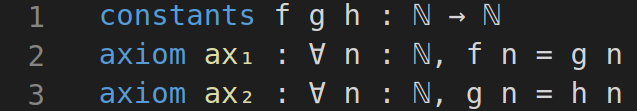
\includegraphics[width=20em]{diagrams/d1}}}
\end{equation*}
The first line (1) declares the existence of three functions $f$, $g$ and $h$, each sending natural numbers to natural numbers. Line (2) then asserts (under the name \xx{$\text{ax}_\text{1}$}) that it is known that $f(n) = g(n)$ for every $n \in \NN$. Line (3) asserts the analogous fact \xx{$\text{ax}_\text{2}$} for the pointwise equality of $g$ and $h$. We now introduce a theorem to be proved:
\begin{equation*}
  \colorbox{bg}{\makebox[0.9\linewidth][l]{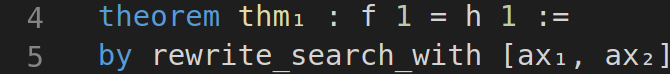
\includegraphics[width=21em]{diagrams/d2}}}
\end{equation*}
Line (4) declares that we intend to prove a theorem \xx{$\text{thm}_\text{1}$} which claims that $f(1) = h(1)$. On line (5) we invoke our general machinery, instructing Lean to perform pair-exploration using the rewrite lemma list $L = [\xx{$\text{ax}_\text{1}$},\xx{$\text{ax}_\text{2}$}]$.

This code sample compiles and executes without error, and this indicates that \xx{rewrite\_search} successfully obtains a proof. Upon request, the interactive editor panel reports the rewrite steps which were performed (written in valid Lean language itself), and this is accompanied by the following interactive force-directed graph (of which we provide only an image capture) depicting the entire rewrite graph which was explored.
\begin{equation*}
  \colorbox{bg2}{\makebox[26em][c]{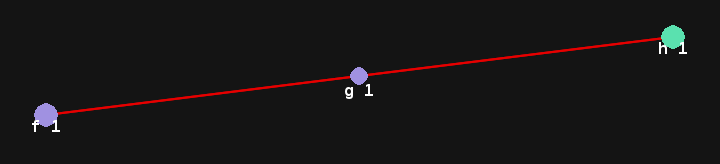
\includegraphics[width=26em]{diagrams/d3}}}
\end{equation*}
The two larger vertices represent the original left- and right-hand expressions, and the colour of intermediary vertices (in this case of which there is one) represents which of the two larger vertices they were first obtained from by rewriting. Of course, in this case the actual proof obtained is entirely trivial, requiring (as shown) a single rewrite of the left-hand side $f(1)$ by \xx{$\text{ax}_\text{1}$}, and then again by \xx{$\text{ax}_\text{2}$}. We now turn to some real examples.

Throughout all of the following examples, a set $L$ of rewrite lemmas from the ambient interactive Lean session have been implicitly tagged. However, we stress that these collections of lemmas were not crafted specifically for the purpose of being sufficient to solve the examples we provide, but instead are defined globally throughout the projects they have been extracted from and have been assembled for the sole purpose of developing the Lean library to which they belong efficiently and concisely.

\subsection{Category theory}

Invocations of \xx{rewrite\_search} have been found to be particularly convenient when developing a from-first-principles category theory library\footnote{This library is available on-line at \url{https://github.com/semorrison/lean-category-theory}.} in Lean. In this context, one often wants to make a construction via specifying the necessary data, where formally a list of conditions which this data must satisfy should also be verified. For example, when defining a functor between categories it might be desirable to specify only what the functor should do on morphisms, leaving well-definedness on the objects and actual functoriality as ``self-evident''---as would certainly be done when communicating to other human mathematicians. Of course when higher-level constructions such as even just monoidal categories or symmetric monoidal functors are to be specified, the list of necessary conditions to be formally checked can grow very rapidly.

Lean's metaprogramming features allow in many situations these extraneous additional proof obligations to be omitted in their entirety, with a request to generate them silently being made a (user-specified) tactic such as \xx{rewrite\_search}. In this setting, \xx{rewrite\_search} has proved very convenient in practise.

A typical example is that of proving that the composition of two equivalences of categories is an equivalence---an equivalence $\mC \cong \mD$ being the data of a functor $F : \mC \to \mD$, a functor $G : \mD \to \mC$, and natural isomorphisms $\alpha : F G \to \id$ and $\beta : G F \to \id$. The Lean code required to define such a composition and generate a formal proof that all of the necessary conditions are satisfied (that each natural transformation $\alpha$ and $\beta$ is an isomorphism and actually natural, for example), is specified fully\footnote{Admittedly, we have used a shorthand notation defined in the ambient category theory library to specify the compositions which give the components of the needed natural isomorphisms.} in the following code snippet.
\begin{equation*}
  \colorbox{bg}{\makebox[.75\linewidth][c]{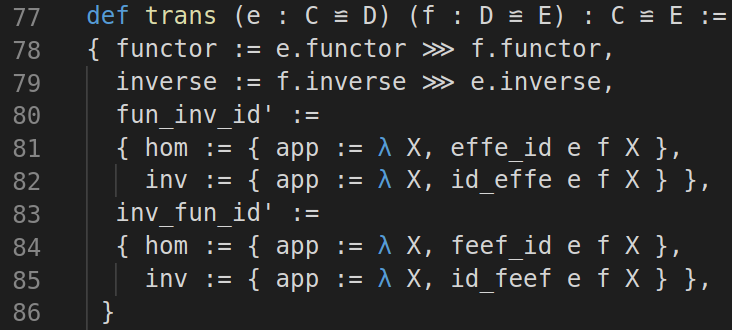
\includegraphics[width=.7\linewidth]{diagrams/d3b}}}
\end{equation*}
Note here that no explicit call to \xx{rewrite\_search} has been made, since the generic mechanism for determining omitted proofs has been invoked.

This is obviously much more concise than explicitly specifying the eight separate proofs of sub-facts which were necessary in order for the Lean-kernel to accept this definition---in fact, with ``trace-mode'' activated and the default parameter values $N_\text{p} = \infty$ and $N_\text{r} = 10$, the following data is reported:
\begin{center}
  \begin{tabular}{c c c c}
    \toprule
    Proof number & \expr{}s seen & \expr{}s visited & Rewrites used\\\midrule
1 & 22 & 10 & 7\\
2 & 91 & 29 & 16\\
3 & 46 & 18 & 10\\
4 & 14 & 6 & 4\\
5 & 22 & 10 & 7\\
6 & 91 & 29 & 16\\
7 & 46 & 18 & 10\\
8 & 14 & 6 & 4\\\bottomrule
  \end{tabular}
\end{center}
The ``rewrites used'' column gives the number of rewrites which were actually used in the final proof. Thus explicitly specifying each of these rewrite lemmas and their order of use would have very significantly---and essentially pointlessly---obfuscated an otherwise routine mathematical definition (especially considering the fact that proofs 1-to-4 and 5-to-8 were completely analogous symmetrical versions of each other).

The different performance impacts of centre-of-mass, SVM, and the unweighted edit-distance metrics are very marginal in this example, and the following one.
Distinguishing between the centre-of-mass and SVM weightings on either side of a slash ``/'', we have the following similar results to those given above:
\begin{center}
  \begin{tabular}{c c c c}
    \toprule
    Proof number & \expr{}s seen & \expr{}s visited & Rewrites used\\\midrule
    1 & 21/22 & 9/10 & 7/7\\
    2 & 86/93 & 28/30 & 17/17\\
    3 & 41/43 & 16/16 & 10/10\\
    4 & 14/14 & 6/6 & 4/4\\
    5 & 21/22 & 9/10 & 7/7\\
    6 & 86/93 & 28/30 & 17/17\\
    7 & 41/43 & 16/16 & 10/10\\
    8 & 14/14 & 6/6 & 4/4\\\bottomrule
  \end{tabular}
\end{center}

This can happen for example when a complex composition of morphisms is to be shown equal to the identity, wherein very little can be gleaned by comparing other derived complicated compositions of morphisms with the single identity morphism. The distinction between the weighting strategies is much more prominent in other areas of the category theory library, and (as we shall see) in other problem domains.

We conclude by examining a proof in Lean that a functor $F : \mC \to \mD$ which is part of an equivalence is necessarily full. This result is encoded in the following code snippet (which is excerpted from a file which includes some other facts about equivalences).
\begin{equation*}
  \colorbox{bg}{\makebox[.85\linewidth][c]{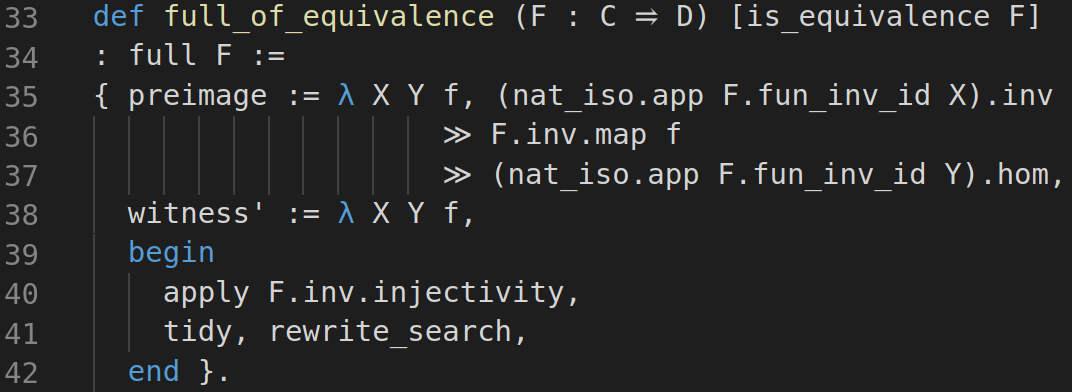
\includegraphics[width=.85\linewidth]{diagrams/d4}}}
\end{equation*}
Notably, on line (40) we have inserted a call to \xx{apply, $\ldots$} in order to hint that faithfulness of one of the functors involved in the equivalence will be critical in the proof (greatly reducing the duration of the search). On the following line we proceed an invocation of \xx{rewrite\_search} by a meta-tactic \xx{tidy}, which by unfolding definitions just simplifies our goal into a single equality to be solved. We have configured \xx{rewrite\_search} in this case to use an SVM classifier metric with $N_\text{p} = 3$ and $N_\text{r} = 10$.

Below we give a visualisation of the search graph built throughout execution of the pair-exploration algorithm, where it is easily seen that the route taken by \xx{rewrite\_search} is very efficient (the actual rewrites which were used are given in red---and efficient at least in the sense that very few ``dead-end'' rewrites have been considered).
\begin{equation*}
  \colorbox{bg2}{\makebox[32em][c]{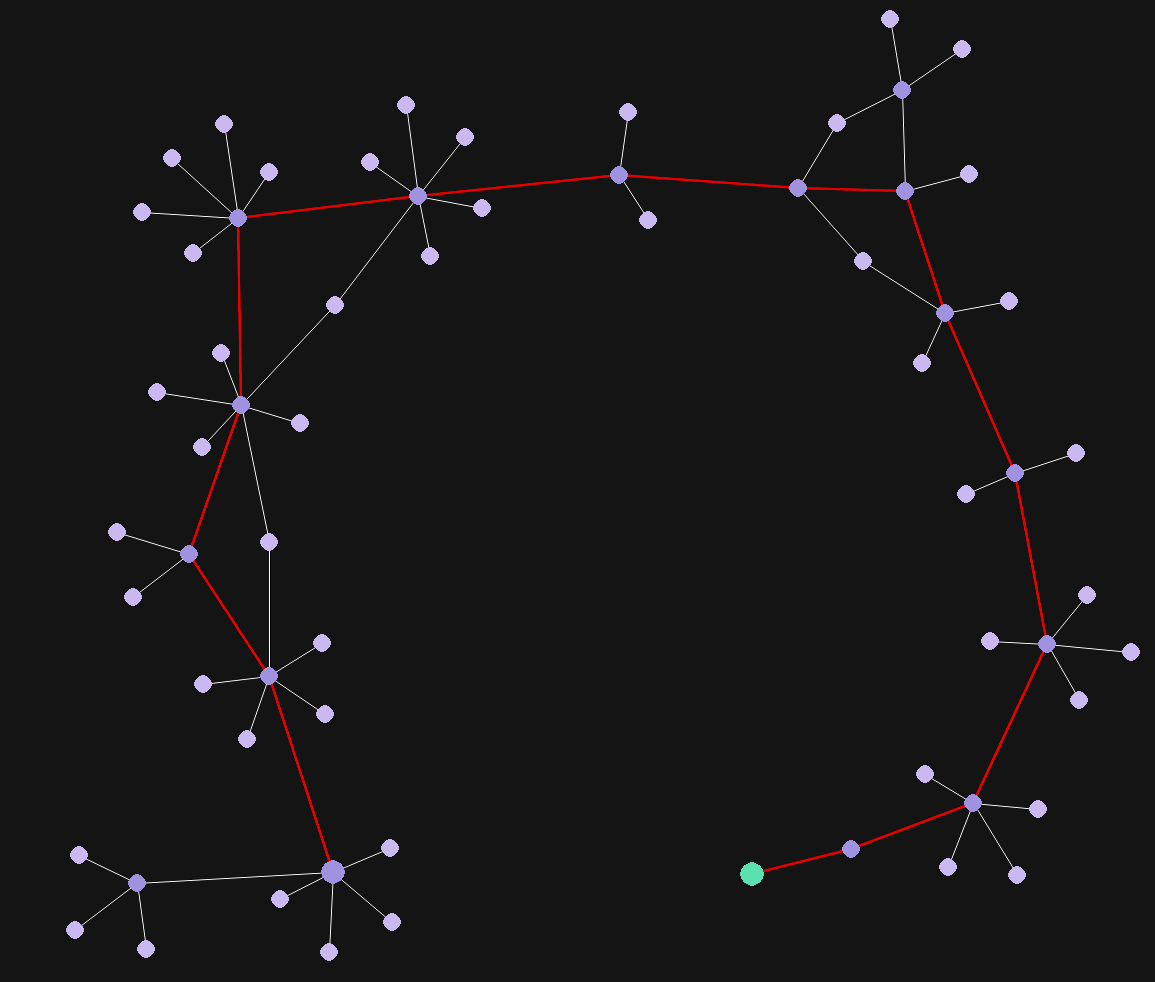
\includegraphics[width=32em]{diagrams/d5}}}
\end{equation*}
It is very important to stress in this instance that the true rewrite graph is infinite, and the true degree of many vertices is approximately 10 (a reduced pop-size parameter limited this number during the actual search). Below we give a continuation of the previous graph, including additional grey vertices which were not even found during the search (but nonetheless were identified by chance after forcing a more complete examination of the rewrite graph for a few minutes) being included.
\begin{equation*}
  \colorbox{bg2}{\makebox[32em][c]{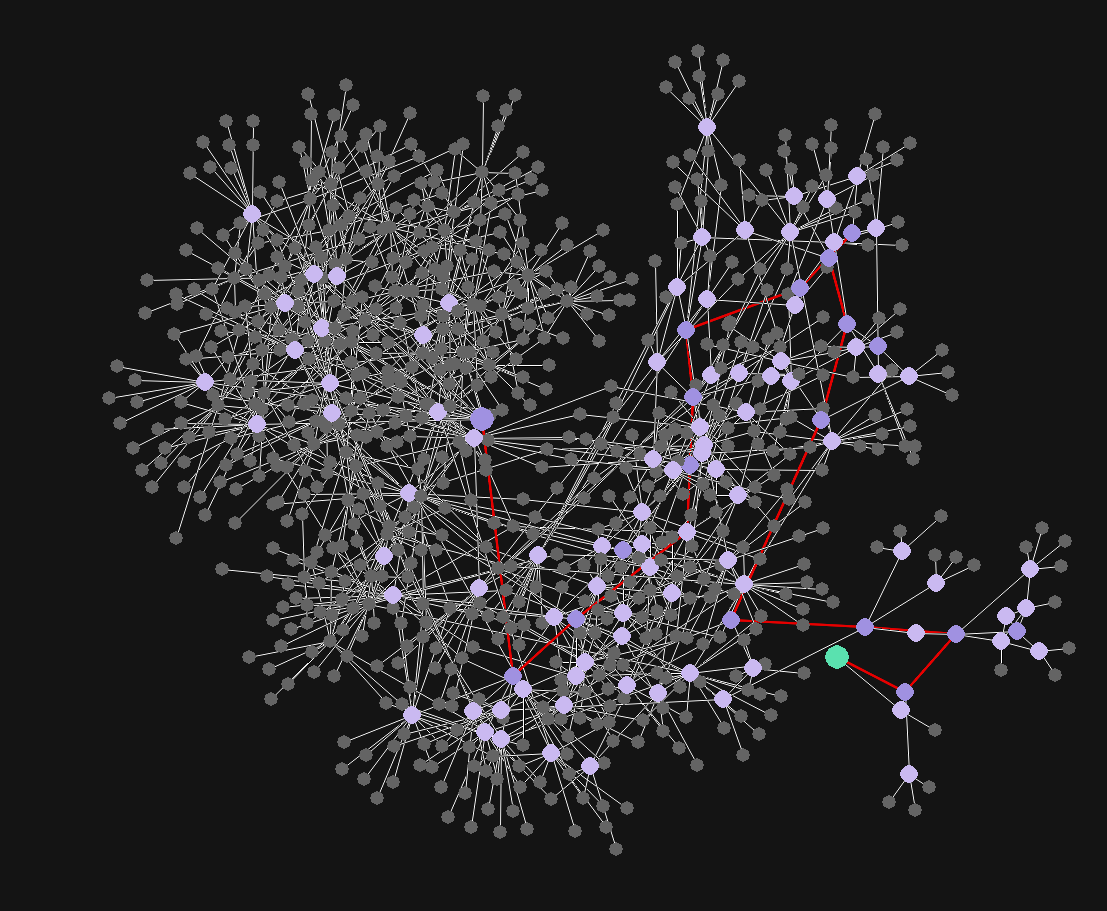
\includegraphics[width=32em]{diagrams/d6}}}
\end{equation*}

\subsection{Arithmetic}

Our pair-exploration algorithm for solving general equational lemmas is automatically suited (or at least applicable) to simplifying equations in arithmetic. For example, the \xx{rewrite\_search} tactic complements ``equation normalisation'' tactics present in Lean's standard library, which are able to solve certain classes of problems quickly but cannot handle arbitrary division, for example---\xx{rewrite\_search} is necessarily much more robust by design. If \xx{rewrite\_search} were able to prove an equational lemma in roughly the same time as it would take to determine that the lemma belongs to a class which can solved by a more efficient algorithm, then the utility of \xx{rewrite\_search} as a general purpose interactive Lean tactic would obviously be further improved.

Consider the example of proving the (completely arbitrary) equational lemma
\begin{equation*}
  (a \times (b + c + 1) / e) \times d = a \times (b / e \times d) + a \times (1 / e \times d) + a \times (c / e \times d)
\end{equation*}
for $a, b, c, d, e$ all rational numbers (and $e$ nonzero). In Lean we would specify this lemma via:
\begin{equation*}
  \colorbox{bg}{\makebox[.95\linewidth][c]{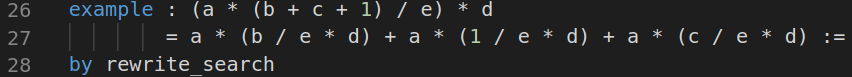
\includegraphics[width=.95\linewidth]{diagrams/d6b}}}
\end{equation*}
The setting of arithmetic provides an excellent example of the utility of centre-of-mass and SVM weighted edit-distance metrics over the standard unweighted metric.

Fix the parameters $N_\text{p} = 10$ and $N_\text{r} = 10$ (we increase $N_\text{p}$ compared to the previous section to eliminated the ``blinder'' effect at low setting has on performance in typical arithmetic problems). Then an unweighted search sees a total of 556 \expr{}s and visits 89, in order to obtain a proof using 19 rewrites. On the other hand a centre-of-mass weighted search sees 180 \expr{}s, visits 25, and finds a proof using 17 rewrites, while an SVM weighted search has the very similar performance of 187 \expr{}s seen, 25 visited, and a proof of length 18. There is a corresponding factor-of-ten reduction in execution time as a consequence. This makes use of an unweighted pair-exploration search for this purpose quite impractical, while the weighted variants enjoy convenient interactive behaviour.

\subsection{Hypercube complete graphs}

Finally, we will examine a much more contrived problem domain compared to those we have just seen, but which will allow us to demonstrate the advantages of an A*-like metric in a simple (and extreme) case. In this example we will not provide the Lean code required to explicitly construct\footnote{It being too unwieldy and also computer generated. The \textit{Mathematica}\texttrademark{} 11.0 notebook used to generate the example can be found at \url{https://github.com/semorrison/lean-tidy/blob/master/test/rewrite_search_cube_axioms.nb}.} the interactive context in which we will invoke \xx{rewrite\_search}---we will be content to just describe it.

We define three functions $f$, $g$, and $h$, all maps $\NN \times \NN \times \NN \to \NN$. We then introduce axioms of the form
\begin{align*}
  &\forall a, b, c \in \NN : f(a, b, c) = f(\alpha, b, c)\\
  &\forall a, b, c \in \NN : f(a, b, c) = f(a, \beta, c)\\
  &\forall a, b, c \in \NN : f(a, b, c) = f(a, b, \gamma)
\end{align*}
for all possible $\alpha, \beta, \gamma \in X = \{1, 2, 3\}$. We proceed reproducing the resulting set of axioms twice more; replacing $f$ everywhere with $g$, and then again with $h$.

The result is that these axioms specify three disjoint complete graphs each on $\lvert X \rvert^3 = 27$ vertices, with one graph corresponding to each of $f$, $g$, and $h$ (the first of which has vertices $f(a, b, c)$ for $(a, b, c) \in X^3$, and analogously for $g$ and $h$). We then additionally impose the axioms
\begin{equation*}
f(2,2,2) = g(3,3,3) \quad \text{and} \quad g(1,1,1) = h(2,2,2).
\end{equation*}
This creates a path from any vertex in any of the complete graphs to any vertex of any other---i.e. combined with the previous axioms asserts that the functions $f$, $g$, and $h$ agree on $X^3$. Our goal will be to prove that $f(1,1,1) = h(1,1,1)$.

This is an interesting toy environment to consider when testing an A*-like metric, since it is possible to perform several rewrites pointlessly meandering within a single complete graph, before finally moving to a vertex in that graph for which one of the two special axioms above permit rewriting into a different complete graph. The purpose of our A*-metric is of course to try to minimise this behaviour and approximate optimality.

In order to maximise the chance of a ``meandering'' route being found due to poor knowledge of the total search graph, we set $N_\text{p} = 1$ and choose a default value of $N_\text{r} = 10$. A direct invocation of \xx{rewrite\_search} using the unweighted edit-distance metric yields the performance 80 \expr{}s seen, 72 \expr{}s visited, 17 rewrites used.

Taking $\alpha = 5$ (an arbitrary, large quantity compared to the standard edit-distance cost of 1) in the definition of the A*-like unweighted edit-distance metric $m^\text{A*}_\alpha$, we instead see the much improved result 80 \expr{}s seen, 76 \expr{}s visited, and only 11 rewrites used in the final proof (this is optimal). Visualising these results, we improved the extremely-meandering path
\begin{equation*}
  \colorbox{bg2}{\makebox[32em][c]{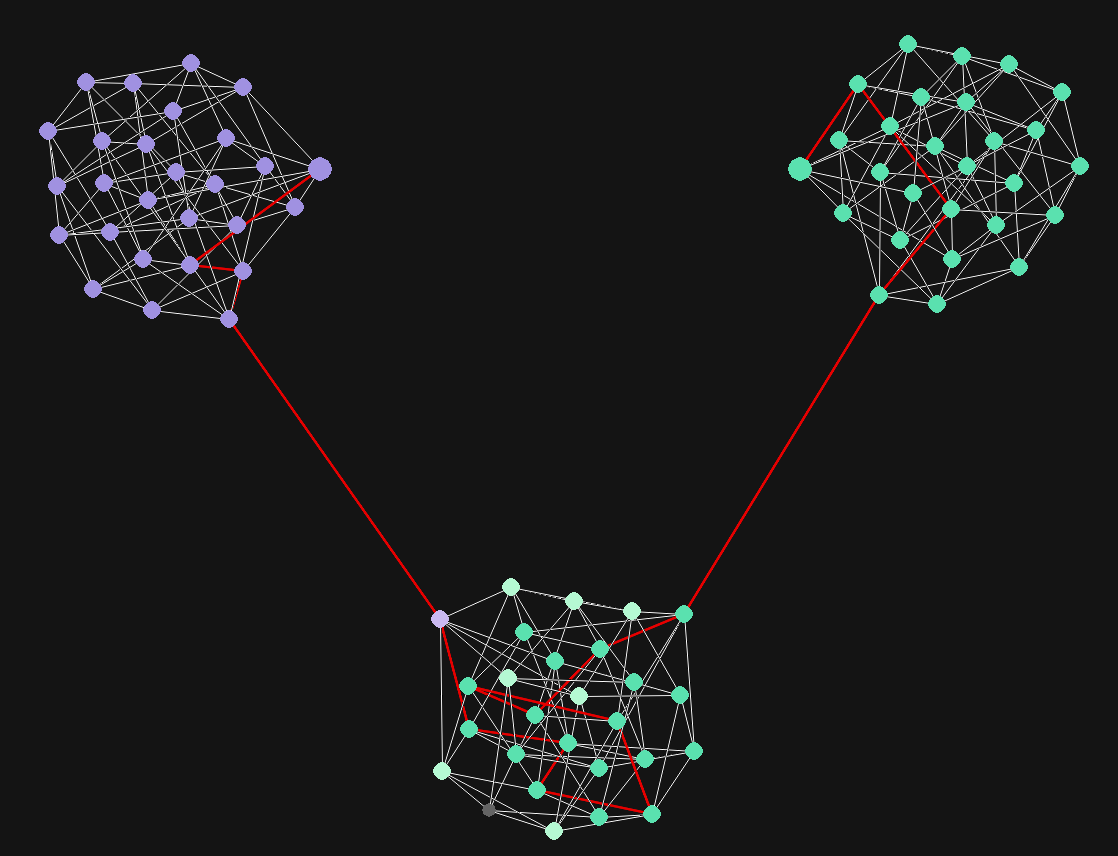
\includegraphics[width=32em]{diagrams/d7}}}
\end{equation*}
into the optimal path
\begin{center}
    \colorbox{bg2}{\makebox[32em][c]{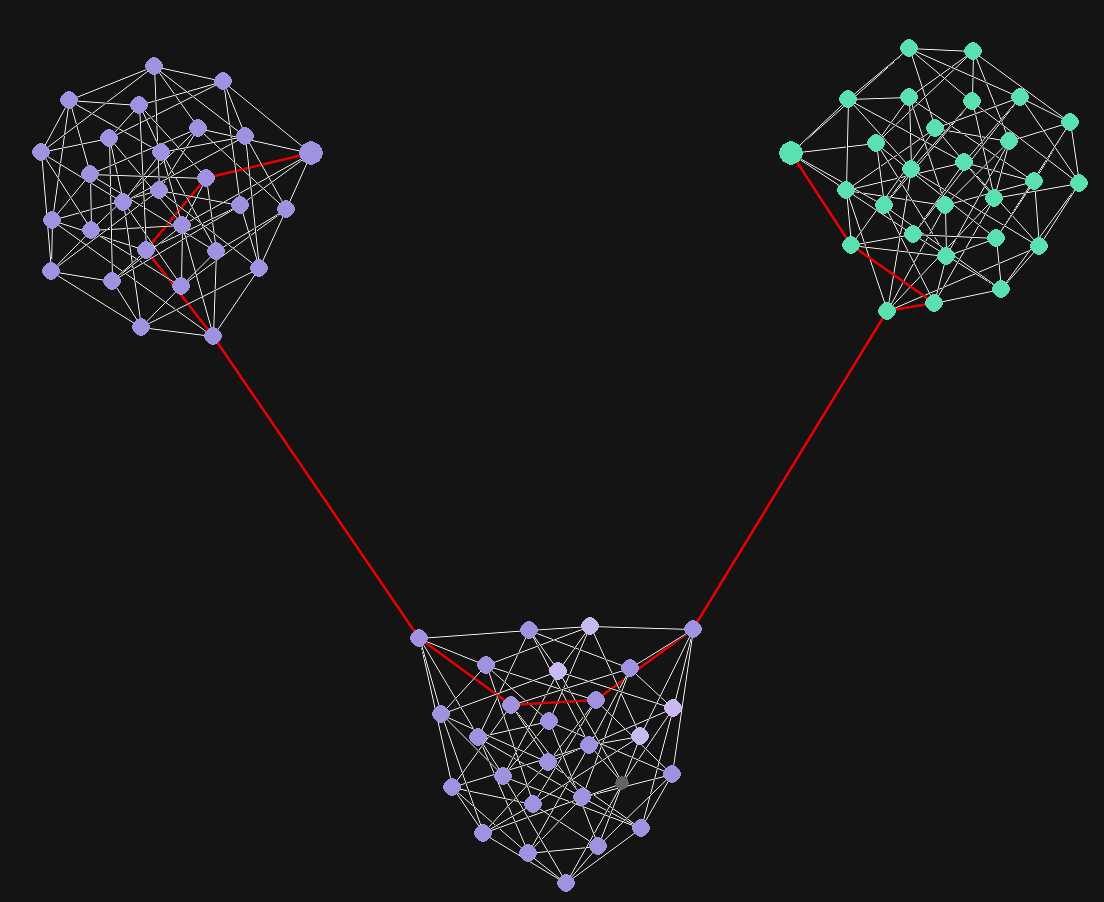
\includegraphics[width=32em]{diagrams/d8}}}.
\end{center}

Because of the relatively high performance impact associated with introducing additional \expr{} vertices to the search graph (and hence the desire to introduce the pop-size parameter $N_\text{p}$), it appears promising to set $N_\text{p} = 1$ and counteract the ``graph blindness'' which is incurred by only revealing a single edge at time by using an A*-like approach such as that which we just gave. The A*-approach also exhibits better performance in terms of fewer total \expr{}s seen for smaller values of $\alpha$, say $\alpha = 1$, at the cost of not producing a precisely-optimal length 11 path (we we find a length 14 path in this case). Performance is seen to improve additionally when a classifier-weighting such as centre-of-mass or SVM is introduced.

Finally, note that the long and meandering 17-rewrite path initially obtained could be reduced to a closer-to-optimal length 14 path by running a shortest-path algorithm on the known rewrite graph when any path whatever connecting the left- and right-hand sides is found---as opposed to simple naive backtracking (the former of which we have implemented in our Lean module and recommend). While overlapping with the advantages of the A*-like metric, we expect that A*-like metrics should also decrease path-lengths in situations where the total rewrite graph is too large and sparse to possibly be fully known---a situation where finding a shortest-path using the resulting rewrite graph at the end of a search would likely be of little benefit.

\section{Future work}

There are many possible directions for future extensions of this work---given its modular nature, each piece can essentially be individually examined and improved on its own. We conclude by giving some recommended directions of further enhancement primarily based on observations made when the algorithm was used in practice.

The fact that our edit-distance calculations are performed on space-tokenized pretty-printed strings is quite a crude procedure, though nonetheless possesses significant power in practical applications (perhaps surprisingly so). Since expressions in Lean are essentially repeated function applications, they possess a natural tree structure which could potentially be exploited for additional information. One possibility is to replace the string-tokenized edit-distance metric with a labelled-tree edit-distance metric, such as that of \cite{pawlik2011rted}.

In practice, it desirable that a search is able to be left to run for some period of time, especially in the case where it is not even known if a rewrite-path between the two input expressions exists. It is therefore desirable that searches lasting a very large number of pair-exploration iterations remain efficient over time. One factor which has been observed to interfere with this efficiency is a build-up of ``stale'' interesting pairs which were found earlier in the search, but where additional progress on the problem had been made since and the pairs would never be revisited. Nonetheless, these pairs remain in the global interesting pair list $P$ and can consume calculation time as each new pair selected from $P$ is compared with each of $P$'s its elements. This problem is particular pertinent in situations where a classifier such as SVM refreshes the weights associated to each token, and therefore all distance estimates as well. Each of the distance estimates for the potentially many ``stale'' pairs must be recalculated in this case, which can be very expensive, in practice even completely pausing the search for a moment. We thus propose that in the interest of performance a strategy for pruning ``stale'' interesting pairs from the list $P$---migrating them to some kind of ``back-up'' list, or just dropping them altogether---be investigated.

An implementation detail of the \xx{rewrite\_search} tactic is that if a maximum number of pair-exploration iterations are exceeded, then the tactic aborts returning an error message. This is necessary to prevent situations where an impossible problem is posed to \xx{rewrite\_search} and leads to an infinite-loop. However, it is often the case that a rewrite-problem is impossible not because the equality it represents is actually false, but because \xx{rewrite\_search} has not been explicitly made aware of a needed rewrite lemma (or this lemma has not yet been proved). It would instead be more desirable if once a maximum number of iterations were reached, the ``goal state''---representing what remains of the theorem to be proved---is replaced with a human-readable simplified version of the equality (i.e. measured by the metric to have smallest distance between its two sides) which was original given as input. This would allow missing lemmas to be more easily identified, and also aid in interactively proving theorems where the complete proof strategy is not already fully known.

Finally, we suggest a direct extension to the pair-exploration algorithm itself which is inspired by human behaviour. Often humans are not only able to recognise that particular terms of one side of an equality should be eliminated (as we attempted to motivate using weighted edit-distances), but they go an additional step to conclude that it suffices to show some number of other equalities of subterms, or of intermediary expressions. These ``conjectured sub-equalities'' are often obtained just by pattern matching, and are frequently those terms most significantly contributing to the edit-distance cost of changing the tokens of one side of the equality to to the other. A general strategy for determining such sub-equalities would be very valuable, both from the perspective of guiding the algorithm and improving performance, and also proving more helpful feedback to an interactive user of the tactic. Tactic users could be informed of the sub-equalities which were determined but could not be discharged automatically, and also the ambient interactive environment could be automatically searched for rewrite lemmas which were not explicitly provided but closely match the conjectured equalities.

\printbibliography


\end{document}
